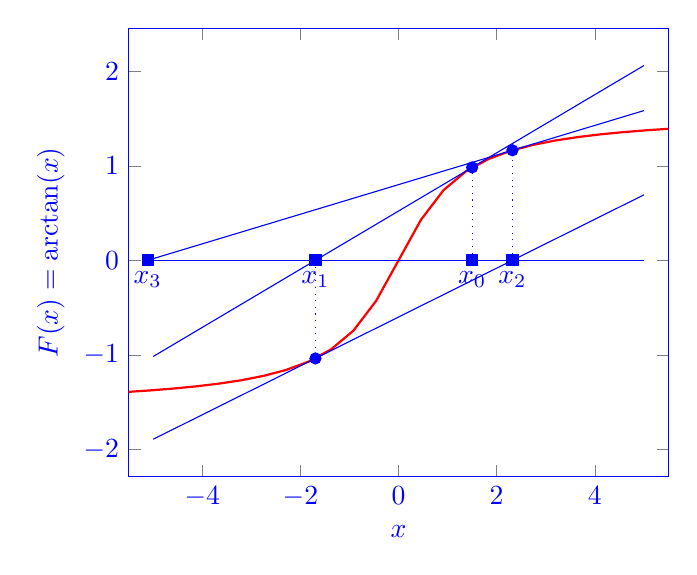
\begin{tikzpicture}[blue]
  \begin{axis}[
      domain=-5.5:5.5, 
      xmin=-5.5, 
      xmax=5.5, 
      xlabel=$x$, 
      ylabel={$F(x)=\arctan(x)$}, 
    ]
    \addplot[thick, red, mark=none] {rad(atan(x))};
    \addplot[mark=none] coordinates {(-5, 0) (5, 0)};
    % x0  
    \addplot[mark=square*] coordinates {(1.5, 0)};
    \addplot[dotted, mark=none] coordinates {(1.5, 0) (1.5, 0.9828)};
    \addplot[mark=*] coordinates {(1.5, 0.9828)};
    \node at (axis cs: 1.5, -0.2) {$x_0$};
    % Tangent
    \addplot[mark=none] coordinates {(-5, -1.017) (5, 2.0597)};
    \addplot[mark=square*] coordinates {(-1.6940796, 0)};
    % Next iterate
    \addplot[dotted, mark=none] coordinates {
      (-1.6940796, 0) (-1.69407960055382, -1.03754635913789)
    };
    \addplot[mark=*] coordinates {(-1.69407960055382, -1.03754635913789)};
    \node at (axis cs: -1.69407960055382, -0.2) {$x_1$};
    % Tangent
    \addplot[mark=none] coordinates {
      (-5, -1.89181017373556) (5, 0.692232124260424)
    };
    \addplot[mark=square*] coordinates {(2.32112696143839, 0)};
    % Next iterate
    \addplot[dotted, mark=none] coordinates {
      (2.32112696143839, 0) (2.32112696143839, 1.16400204242198)
    };
    \addplot[mark=*] coordinates {(2.32112696143839, 1.16400204242198)};
    \node at (axis cs: 2.32112696143839, -0.2) {$x_2$};
    % Tangent
    \addplot[mark=none] coordinates {
      (-5, 0.017860744931861) (5, 1.58338652194274)
    };
    \addplot[mark=square*] coordinates {(-5.11408783677751, 0)};
    \node at (axis cs: -5.11408783677751, -0.2) {$x_3$};
  \end{axis}
\end{tikzpicture}
